\documentclass{beamer}

\usepackage{beamerthemesplit}
\usetheme{Singapore} %Copenhagen}
%\usecolortheme{whale}

%\usepackage[T2A]{fontenc}
%\usepackage[utf8]{inputenc}
%\usepackage[russian]{babel}

\usepackage[main=russian,english]{babel}   %% загружает пакет многоязыковой вёрстки
\usepackage{fontspec}      %% подготавливает загрузку шрифтов Open Type, True Type и др.
\defaultfontfeatures{Ligatures={TeX},Renderer=Basic}  %% свойства шрифтов по умолчанию
\setmainfont{Times New Roman} %% задаёт основной шрифт документа
%\usefonttheme{professionalfonts}% SOLUTION
\usefonttheme{serif}

\usepackage{hyperref}
\usepackage{textcomp}
\usepackage{amssymb,amsmath}
%\usepackage{animate}
%\usepackage{longtable}
\usepackage{xcolor}

%\usepackage{pgffor}
\usepackage{enumitem}
\usepackage[export]{adjustbox}

\newcounter{N}

%% Форматирование окружения itemize
%\usepackage{ragged2e}
%\let\olditem\item
%\renewcommand\item{\olditem\justifying}

\usepackage{ mathrsfs }
\newcommand{\Rho}{\mathscr{P}}

\renewcommand{\Re}{\operatorname{Re}}

\newcommand{\argxi}{(\xi^1,\xi^2,\xi^3)}
\newcommand{\argx}{(x^1,x^2,x^3)}

\newcommand{\argxiv}{(\vec{\xi})}
\newcommand{\argxv}{(\vec{x})}


\newcommand{\argxbarn}{(\bar{x}^1,\bar{x}^2,\ldots, \bar{x}^n)}
\newcommand{\argxn}{(x^1, x^2,\ldots, x^n)}

\newcommand{\argtxi}{(t, \xi^1,\xi^2,\xi^3)}
\newcommand{\argtoxi}{(t_0, \xi^1,\xi^2,\xi^3)}

\newcommand{\argtxiv}{(t, \vec{\xi})}
\newcommand{\argtoxiv}{(t_0, \vec{\xi})}


\newcommand{\argtx}{(t, x^1,x^2,x^3)}
\newcommand{\argtox}{(t_0, x^1,x^2,x^3)}

\newcommand{\argtxv}{(t, \vec{x})}
\newcommand{\argtoxv}{(t_0, \vec{x})}


\newcommand{\pd}[2]{\frac{\partial #1}{\partial #2}}
\newcommand{\pdk}[2]{\frac{\partial^2 #1}{\partial #2^2}}

\newcommand{\od}[2]{\frac{d #1}{d #2}}
\newcommand{\odk}[3]{\frac{d^{#3} #1}{d #2^{#3}}}

\newcommand{\grad}{\operatorname{grad}}
\newcommand{\rot}{\operatorname{rot}}
\newcommand{\divo}{\operatorname{div}}

\title[]{Течения вязкой жидкости}

\author[]{ {\em Верещагин Антон Сергеевич}
\\
канд. физ.-мат. наук, старший преподаватель\\
\bigskip
Кафедра аэрофизики и газовой динамики ФФ НГУ}

\usebackgroundtemplate{
\includegraphics[width=\paperwidth]{../img/background.png}}

\begin{document}
	
\frame{\titlepage}


\frame{
	\frametitle{Аннотация}
	\parbox{\textwidth}{

	}
}

\frame{
	\frametitle{Понятие вязкой жидкости}
	
	\begin{columns}
		\begin{column}{0.4\textwidth}
			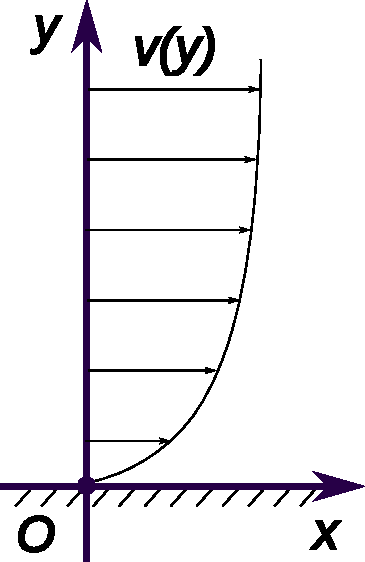
\includegraphics[width=\linewidth]{../img/visc_def.pdf}
		\end{column}
		\begin{column}{0.6\textwidth}
			\begin{exampleblock}{Касательная сила, действующая на стенку}
				\parbox{\textwidth}{
					\[
					\tau= \mu \od{v}{y} = \rho\nu \od{v}{y},
					\]
					здесь $\mu=\rho\nu$ -- коэффициент динамической вязкости;
					$\nu$ --  коэффициент кинематической вязкости; $\rho$ -- плотность.
					

				}
			\end{exampleblock}\pause
		
			\begin{exampleblock}{Размерность коэффициентов вязкости}
				\parbox{\textwidth}{
				\[
					[\mu] = \frac{\text{кг}}{\text{м} \cdot \text{с}},\quad
					[\nu] = \frac{\text{м}^2}{\text{с}}.
				\]
					
				}
			\end{exampleblock}
		
			
		\end{column}
	\end{columns}
}


\frame{
	\frametitle{ Тензор напряжений вязкой несжимаемой жидкости }
	
	\begin{columns}
		\begin{column}{0.3\textwidth}
			\centering\scriptsize
			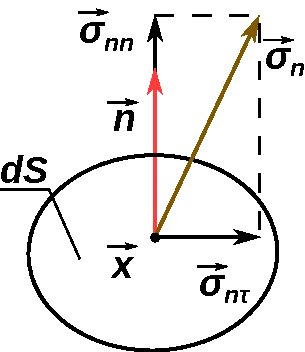
\includegraphics[width=\linewidth]{../img/sigma_decomposition}\\
			
			\medskip
			Разложение напряжения, возникающего в сплошной среде, на тангенциальную и нормальную составляющие
		\end{column}
		\begin{column}{0.7\textwidth}
				\begin{exampleblock}{Связь тензора напряжения и тензора скоростей деформации}
				\parbox{\textwidth}{
					\[
					\sigma = -pI + 2\mu e,
					\]
					где $p$ -- давление; $I$ -- единичный тензор; $e$ -- тензор скоростей деформаций, задаваемый соотношением
					\[
					e_{ij} = \frac{1}{2}\left( \pd{v_i}{x_j}+\pd{v_j}{x_i} \right);
					\]
					$v_i$  -- компоненты вектора скорости ($i=\overline{1,n}$).
				}
			\end{exampleblock}
		\end{column}
	\end{columns}
	

	
}

\frame{
	\frametitle{ Уравнения движения вязкой несжимаемой жидкости }
	
	\begin{exampleblock}{Уравнения Навье-Стокса}
		\parbox{\textwidth}{
			\[
				\divo \vec{v} = 0,
			\]
			\[
				\pd{\vec{v}}{t} + (\vec{v}\cdot\nabla)\vec{v} = -\frac{1}{\rho}\nabla p + \nu \Delta \vec{v} + \vec{f},
			\]
			\[
			c_V\left(\pd{\vec{T}}{t} + (\vec{v}\cdot\nabla)T \right) = \frac{\kappa}{\rho} \Delta T + \frac{2\mu}{\rho} e_{ij}e_{ij},
			\]
			
			\medskip
			\alert{Неизвестные функции}, определённые и дифференцируемые в некоторой области пространства:  $\vec{v}\argtxv$ -- вектор скорости; $p\argtxv$ -- давление; $T\argtxv$ -- температура. 

			\medskip			
			\alert{Константы}: $\rho$ -- плотность; $\nu$ -- коэффициент кинематической вязкости; $\kappa$ -- коэффициент температуропроводности; $e_{ij}$ -- компоненты тензора скоростей деформации; $\vec{f}$ -- вектор внешних сил.
			
		}
	\end{exampleblock}
}

\frame{
	\frametitle{Уравнения движения вязкой несжимаемой жидкости}
	
	\parbox{\textwidth}{
	Система уравнений разбивается на две подсистемы:	
	}
	
	
	\begin{exampleblock}{Уравнения Навье-Стокса}
		\parbox{\textwidth}{
		\[
		\divo \vec{v} = 0,
		\]
		\[
		\pd{\vec{v}}{t} + (\vec{v}\cdot\nabla)\vec{v} = -\frac{1}{\rho}\nabla p + \nu \Delta \vec{v} + \vec{f}.
		\]	
		}
	\end{exampleblock}

	\begin{exampleblock}{Закон динамики температуры}
		\parbox{\textwidth}{
		\[
		c_V\left(\pd{T}{t} + (\vec{v}\cdot\nabla)T \right) = \frac{\kappa}{\rho} \Delta T + \frac{2\mu}{\rho} e_{ij}e_{ij}.
		\]	
		}
	\end{exampleblock}	
	
	\parbox{\textwidth}{
		Решив уравнения Навье-Стокса мы найдём распределение скорости и давления. Зная распределение скорости, из второй части, находится распределение температуры. Дальше будет рассматриваться только \alert{первая часть системы}.
	}
	
	
}

\frame{
	\frametitle{Граничные условия для уравнения Навье-Стокса}
	
	\begin{columns}
		\begin{column}{0.5\textwidth}
			\begin{exampleblock}{Условия на неподвижной границе}
			\parbox{\textwidth}{
			\centering
			\medskip
			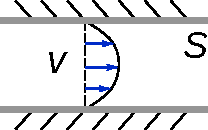
\includegraphics[width=0.7\linewidth]{../img/motionless_bound}

			\bigskip
			Кинематическое условие:
			\[
			\vec{v}|_S = 0.
			\]

			}
			\end{exampleblock}
		\end{column}\pause
	
		\begin{column}{0.5\textwidth}
			\begin{exampleblock}{Условие на подвижной границе}
				\parbox{\textwidth}{
					
					\centering
					\medskip
					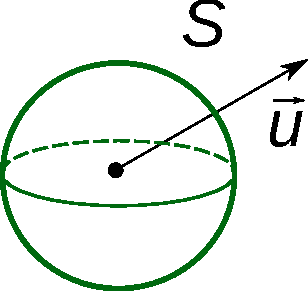
\includegraphics[width=0.5\linewidth]{../img/moving_rigid_bound}
					
					\bigskip
					Кинематическое условие:
					\[
					\vec{v}|_S = \vec{u}.
					\]
					
				}
			\end{exampleblock}
			
		\end{column}
	\end{columns}\pause
	
	\parbox{\textwidth}{
	\centering
	Такого вида граничные условия называются условиями \alert{<<прилипания>>}.
	}
	
	
}

\frame{
	\frametitle{Граничные условия для уравнения Навье-Стокса}
	
	\begin{exampleblock}{Условия на свободной границе}
		\parbox{\textwidth}{
		\begin{columns}
			\begin{column}{0.5\textwidth}
				\scriptsize
				\centering
				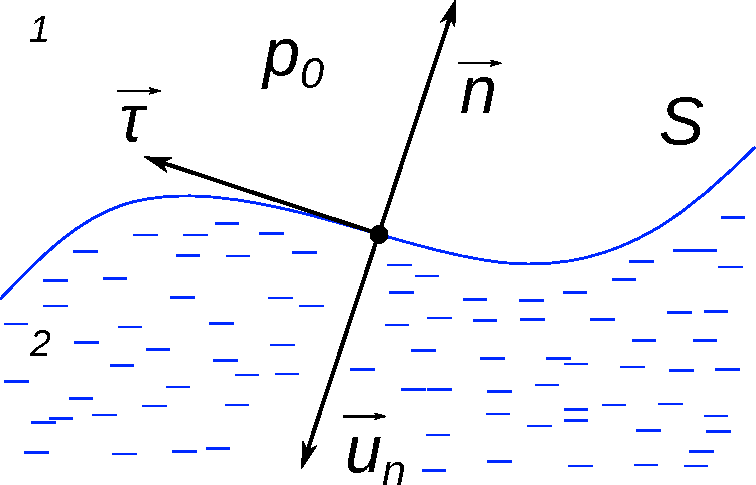
\includegraphics[width=0.7\linewidth]{../img/free_bound}
				
				\medskip
				1 -- воздух (газ); 2 -- вязкая жидкость
			\end{column}
			\begin{column}{0.5\textwidth}
			Кинематическое условие:
			\[
			v_n|_S = u_n.
			\]
			
			\medskip
			Динамические условия:
			\[
			\vec{n}\cdot\sigma|_S= p|_S = p_0,
			\]
			\[
			\vec{\tau}\cdot\sigma|_S = 0.
			\]

				
			\end{column}
		\end{columns}	
		}
	\end{exampleblock}
	
}

\frame{
	\frametitle{Уравнения Навье-Стокса в декартовой системе координат}
%	\begin{exampleblock}{}
%	\parbox{\textwidth}{
%				
		\[
			\pd{v_x}{x}+\pd{v_y}{y}+\pd{v_z}{z} = 0,
		\]
		\[
		\pd{v_x}{t} + 
		v_x \pd{v_x}{x} + v_y \pd{v_x}{y} + v_z \pd{v_x}{z} = 
		X -\frac{1}{\rho}\pd{p}{x} + 
		\nu \left(\pdk{v_x}{x} + \pdk{v_x}{y}+ \pdk{v_x}{z} \right),
		\]
		\[
		\pd{v_y}{t} + 
		v_x \pd{v_y}{x} + v_y \pd{v_y}{y} + v_z \pd{v_y}{z} = 
		Y -\frac{1}{\rho}\pd{p}{y} + 
		\nu \left(\pdk{v_y}{x} + \pdk{v_y}{y}+ \pdk{v_y}{z} \right),
		\]
		\[
		\pd{v_z}{t} + 
		v_x \pd{v_z}{x} + v_y \pd{v_z}{y} + v_z \pd{v_z}{z} = 
		Z -\frac{1}{\rho}\pd{p}{z} + 
		\nu \left(\pdk{v_z}{x} + \pdk{v_z}{y}+ \pdk{v_z}{z} \right).
		\]

%	}
	
%	\end{exampleblock}
}




\frame{
	\frametitle{ Литература }
	\begin{itemize}[partopsep=1pt,label=\textbullet]
		\item 
		{\em Кочин~Н.~Е., Кибель~И.~А., Розе~Н.~В.} Теоретическая гидромеханика. М.:Гос. издат. физ.-мат. лит., 1963.
		\item {\em Валландер~С.~В.} Лекции по аэрогидромеханике. Учеб. пособие. Л., Изд-во Ленингр. ун-та, 1978. 
	\end{itemize}
}

\end{document}
